\documentclass[12pt,b5paper]{ltjsarticle}

%\usepackage[margin=15truemm, top=5truemm, bottom=5truemm]{geometry}
\usepackage[margin=15truemm]{geometry}
\usepackage{graphicx}
\usepackage{amsmath,amssymb}
%\pagestyle{empty}
\pagestyle{headings}

\begin{document}


$\mathbb{R}^2$上で点$(2,0)$と$(-2,0)$からの距離の差が$2$となる
点集合(双曲線)を、
$\mathbb{R}^2$に以下の$2$つの距離が与えられた場合に
それぞれ求めよ。
\begin{enumerate}
 \item $d_1((x_1,x_2), (y_1,y_2)) = \lvert x_1 - y_1\rvert + \lvert x_2 -y_2\rvert$
 \item $d_2((x_1,x_2), (y_1,y_2)) = \max\{\lvert x_1 - y_1\rvert , \lvert x_2 -y_2\rvert\}$
\end{enumerate}

\hrulefill

点$(x,y)$と 点$(2,0)$の距離 と
点$(x,y)$と 点$(-2,0)$の距離 を考え、
この2つの距離の差が $2$ となるように$(x,y)$の軌跡を考える。

\dotfill

\begin{enumerate}
 \item
      \begin{align}
       d_1((x,y), (2,0)) =& \lvert x - 2\rvert + \lvert y -0\rvert
       = \lvert x - 2\rvert + \lvert y\rvert\\
       d_1((x,y), (-2,0)) =& \lvert x + 2 \rvert + \lvert y -0\rvert
       = \lvert x + 2 \rvert + \lvert y \rvert
      \end{align}
      であるので、これらの距離の差はどちらが大きいかで次の2つを考えられる。
      \begin{align}
       \label{neg}
       d_1((x,y), (2,0)) - d_1((x,y), (-2,0))
        =& \lvert x - 2\rvert - \lvert x + 2\rvert\\
       \label{pos}
       d_1((x,y), (-2,0)) - d_1((x,y), (2,0))
       =& \lvert x + 2\rvert - \lvert x - 2\rvert
      \end{align}
      (\ref{neg})の式が正の場合を考える。
      この時、$x<0$である。
      これは$\lvert x - 2\rvert > \lvert x + 2\rvert$ より
      両辺を2乗すると得られる。

      絶対値を外すため2乗をし式を整理する。
      \begin{gather}
       \lvert x - 2\rvert - \lvert x + 2\rvert =2\\
       x^2-4x+4 -2\lvert x^2 - 4\rvert + x^2+4x+4=4\\
       x^2+2 =\lvert x^2 - 4\rvert\\
       (x^2+2)^2 =(x^2 - 4)^2\\
       (x^2+2)^2 -(x^2 - 4)^2=0\\
       6(2x^2-2)=0\\
       x=\pm 1
      \end{gather}
      (\ref{neg})の式の場合、$x<0$より$x=-1$となる。
      
      (\ref{pos})の式の場合も同様に考えると$x=1$となる。

      よってこの場合の軌跡は$x=\pm 1$の2本の直線を表す。

%     \begin{figure}
      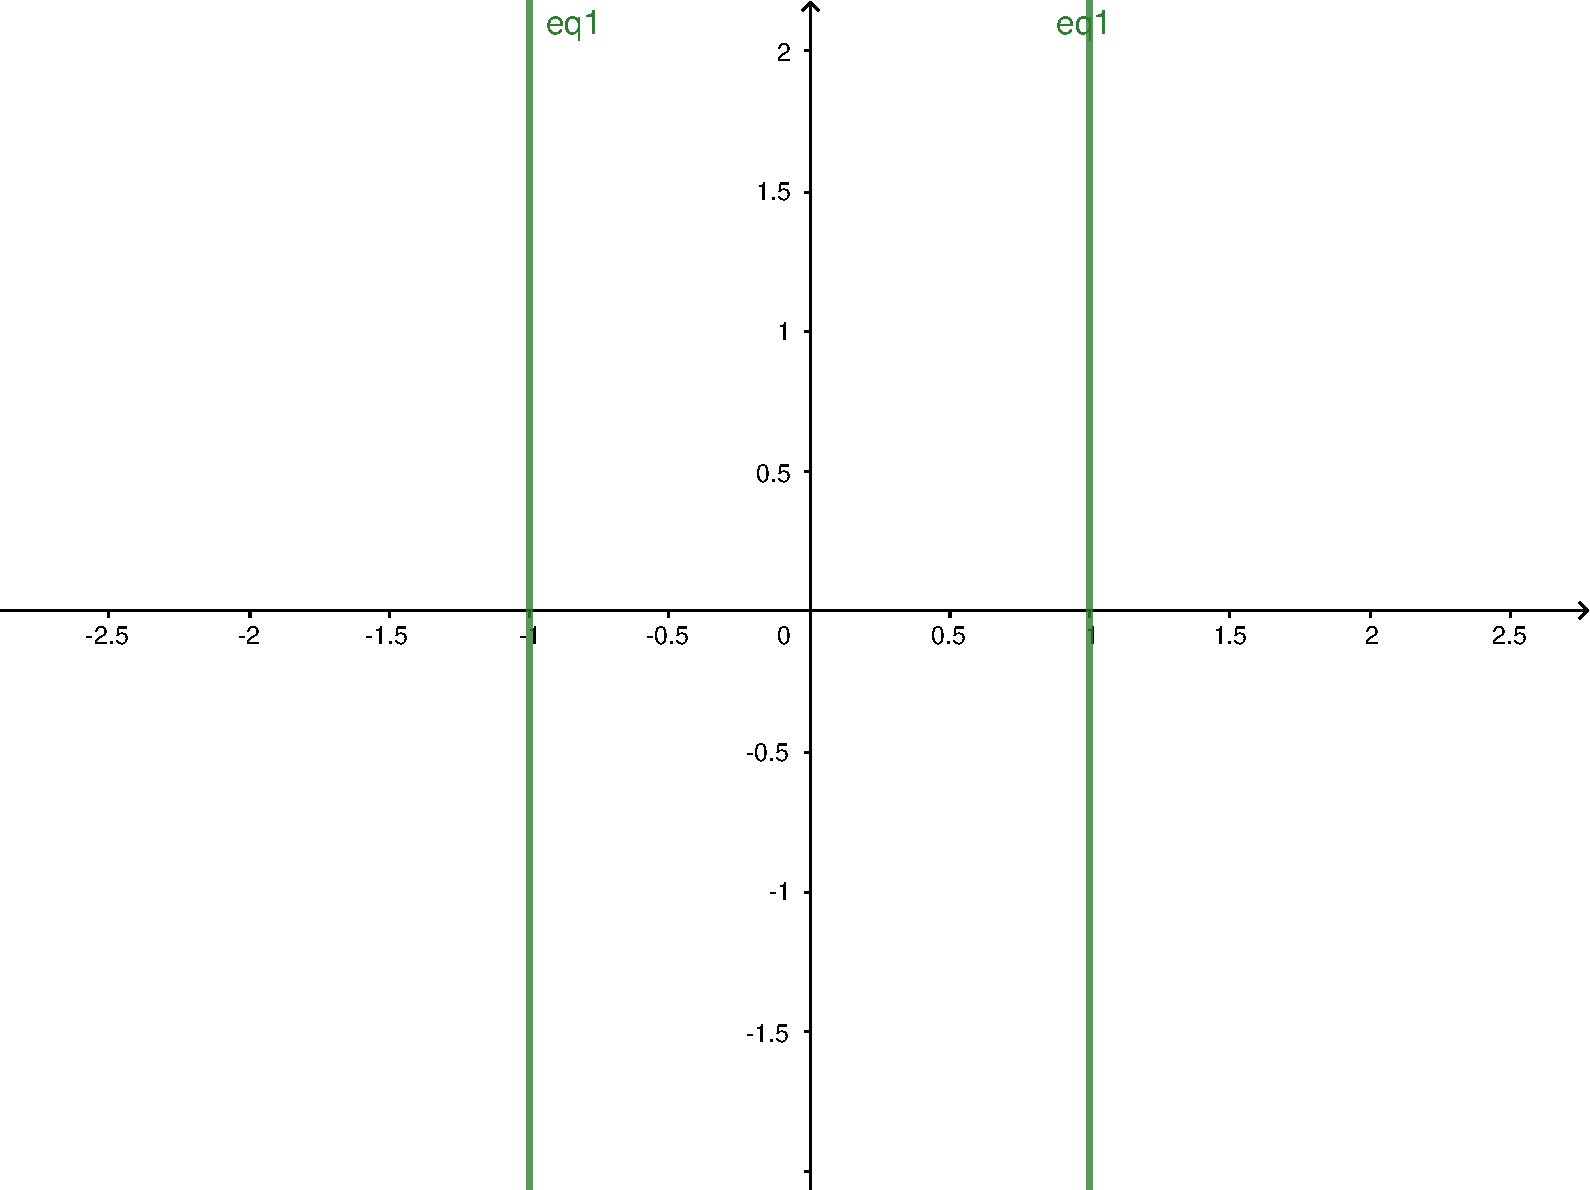
\includegraphics[width=300pt]{orbit_1.pdf}
%     \end{figure}

\dotfill

 \item
      この距離は次のようになる。
      \begin{align}
       d_2((x,y), (2,0)) =& \max\{\lvert x - 2\rvert , \lvert y \rvert\}\\
       d_2((x,y), (-2,0)) =& \max\{\lvert x + 2 \rvert , \lvert y \rvert\}
      \end{align}
      それぞれ$\max$により大きいほうが距離となる。

      問題は距離の差が2である時とあるので、
      考える式は次の2つである。
      \begin{gather}
       \label{pro2-1}
       d_2((x,y), (2,0)) -  d_2((x,y), (-2,0)) =2\\
       \label{pro2-2}
       d_2((x,y), (-2,0)) -  d_2((x,y), (2,0)) =2
      \end{gather}

      まず、式(\ref{pro2-1})について考える。
      距離の差$ d_2((x,y), (2,0)) -  d_2((x,y), (-2,0)) $は
      次の4つの場合が考えられる。
      \begin{align}
       \label{2-con1}
       \lvert x-2 \rvert -& \lvert x+2 \rvert
       & (\lvert x - 2\rvert > \lvert y \rvert ,\
       \lvert x + 2 \rvert > \lvert y \rvert )\\
       \label{2-con2}
       \lvert x-2 \rvert -& \lvert y \rvert
       & (\lvert x - 2\rvert > \lvert y \rvert ,\
       \lvert x + 2 \rvert \leq \lvert y \rvert )\\
       \label{2-neg}
       \lvert y \rvert -& \lvert x+2 \rvert
       & (\lvert x - 2\rvert \leq \lvert y \rvert ,\
       \lvert x + 2 \rvert > \lvert y \rvert )\\
       \label{2-zero}
       \lvert y \rvert -& \lvert y \rvert
       & (\lvert x - 2\rvert \leq \lvert y \rvert ,\
       \lvert x + 2 \rvert \leq \lvert y \rvert )
      \end{align}

      右側に書かれた条件式より導き出される領域は文末に示してある。

      この時、式(\ref{2-zero}) は 0 となるので 距離の差が2になることはない。
      また、式(\ref{2-neg}) は 条件式に$\lvert x + 2 \rvert > \lvert y \rvert$
      とあるので $\lvert y \rvert - \lvert x+2 \rvert<0$
      であり、距離の差は2にならない。
      この為、実際に考える必要があるのは式(\ref{2-con1})と式(\ref{2-con2})である。

      そこで、式(\ref{2-con1})について考える。
      
      前問より$\lvert x-2 \rvert - \lvert x+2 \rvert =2$を満たすのは$x=-1$である。
      $\lvert x - 2\rvert > \lvert y \rvert$の該当する領域は
      図\ref{f1-1} の表され、
      $\lvert x + 2 \rvert > \lvert y \rvert$の領域は
      図\ref{f2-1} で表されるので、
      式(\ref{2-con1})の条件の示す領域はこの2つの重なった部分となる。
      よって、直線$x=-1$のうち、$-1< y < 1$の部分の線分となる。


      次に、式(\ref{2-con2})について考える。
      
      条件は図\ref{f1-1}と図\ref{f2-2}の示す領域である。
      式は$\lvert x-2 \rvert - \lvert y \rvert = 2$であるので
      2つの絶対値の場合分けを行うと次の4つに分わけられる。
      \begin{align}
%       \lvert x-2 \rvert - \lvert y \rvert = 2\\
       x\geq 2 ,\ y\geq 0\ の時、 &\quad y=x-4\\
       x< 2 ,\ y\geq 0\ の時、 &\quad y=-x\\
       x\geq 2 ,\ y< 0\ の時、 &\quad y=-x+4\\
       x< 2 ,\ y< 0\ の時、 &\quad y=x
      \end{align}

      この4つの式からグラフが次のように描ける。
      \begin{center}
       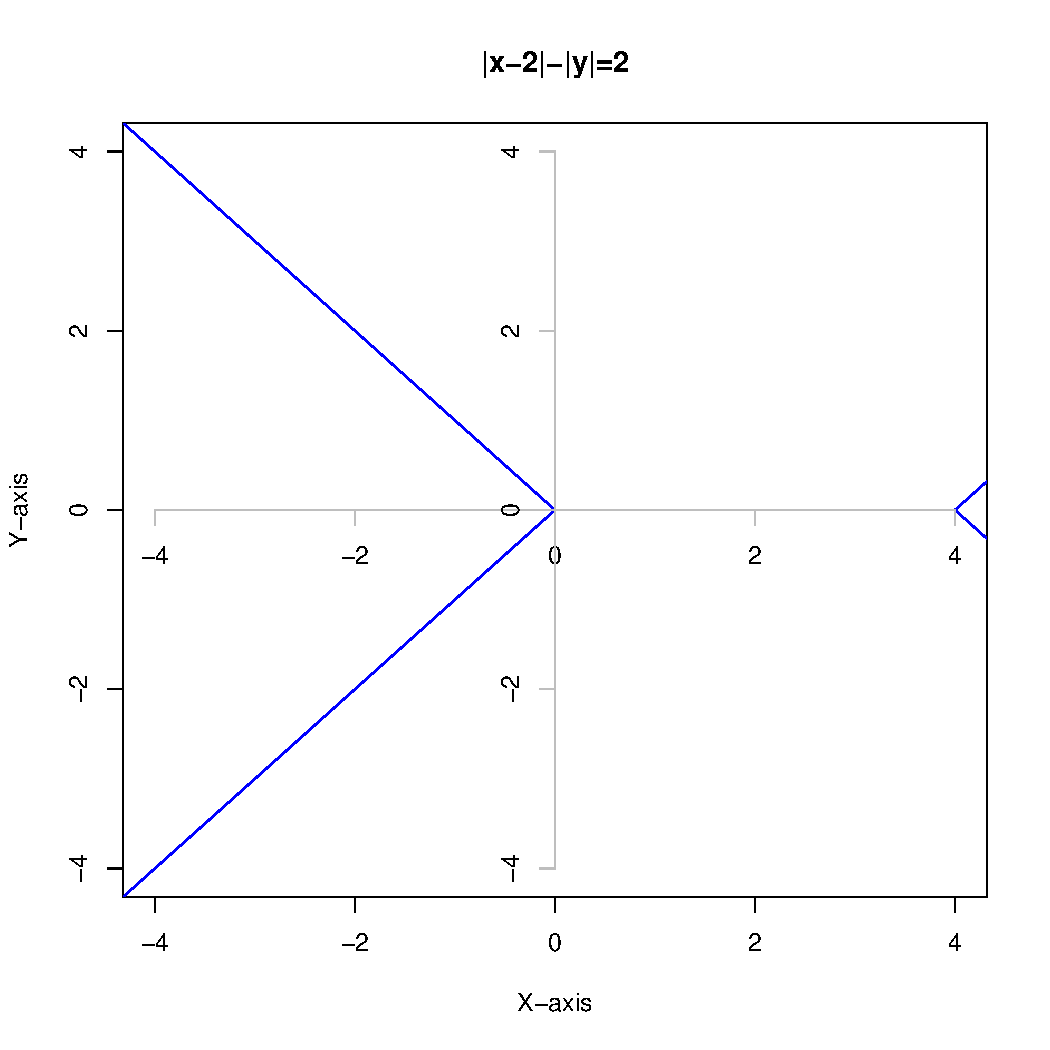
\includegraphics[scale=0.5]{graph.pdf}
      \end{center}
      このグラフは図\ref{f1-1}には全て含まれるので、
      図\ref{f2-2}と重なる部分が条件を満たす軌跡となる。
      グラフの$x\leq 1$の部分が図\ref{f2-2}と重なるので、
      式(\ref{2-con1})の結果である
      直線$x=-1$のうち、$-1< y < 1$の部分の線分
      と合わせると次のグラフが得られる。
      \begin{center}
       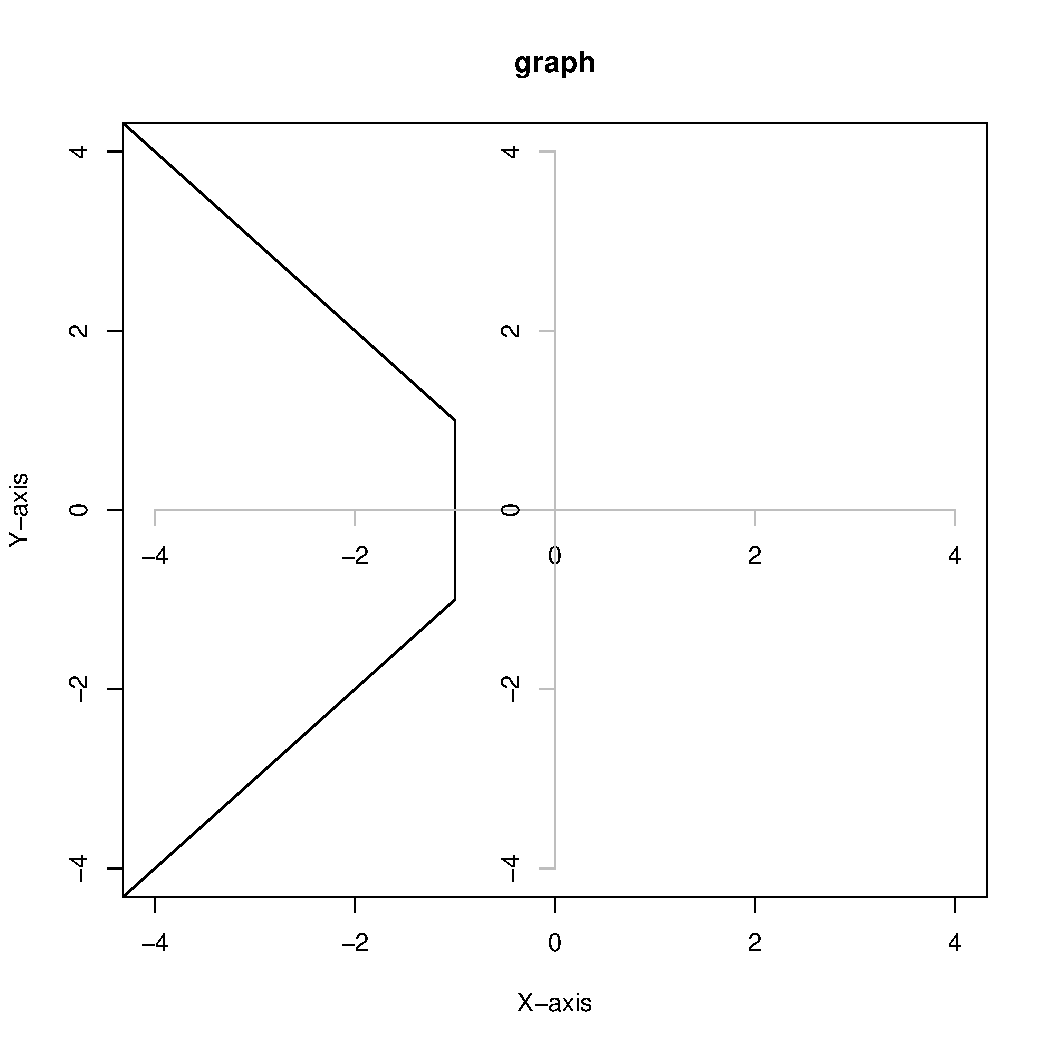
\includegraphics[scale=0.5]{graph_r.pdf}
      \end{center}

      これが式(\ref{pro2-1})の示すグラフとなる。

      同様に式(\ref{pro2-2})も考えると、
      同じようなグラフが求められるので、
      それらをまとめると次のグラフとなる。
      これが距離$d_2$における双曲線である。
      \begin{center}
       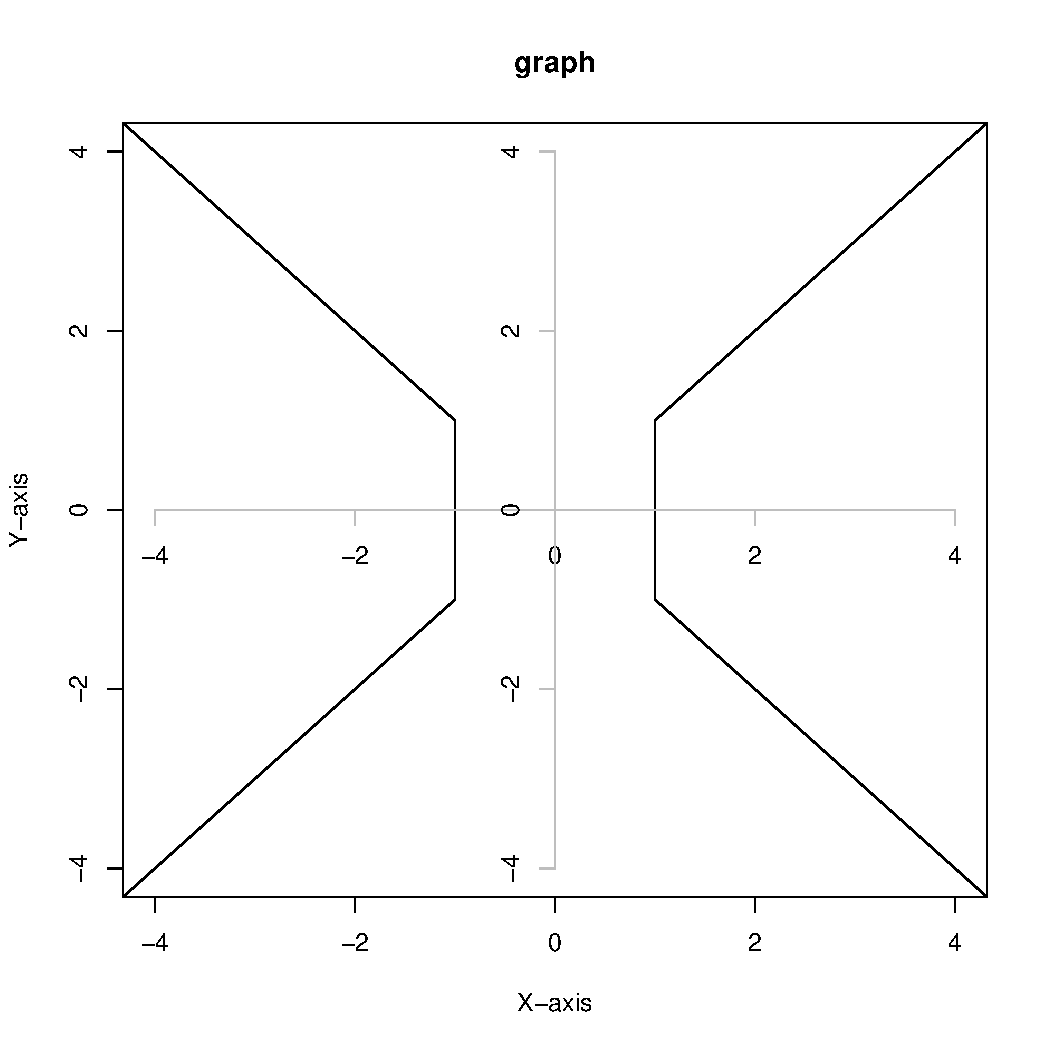
\includegraphics[scale=0.5]{graph_all.pdf}
      \end{center}


      \begin{figure}[h]
       それぞれの不等式が示す領域

       \begin{tabular}{cc}
        \begin{minipage}[c]{200pt}
         \centering
         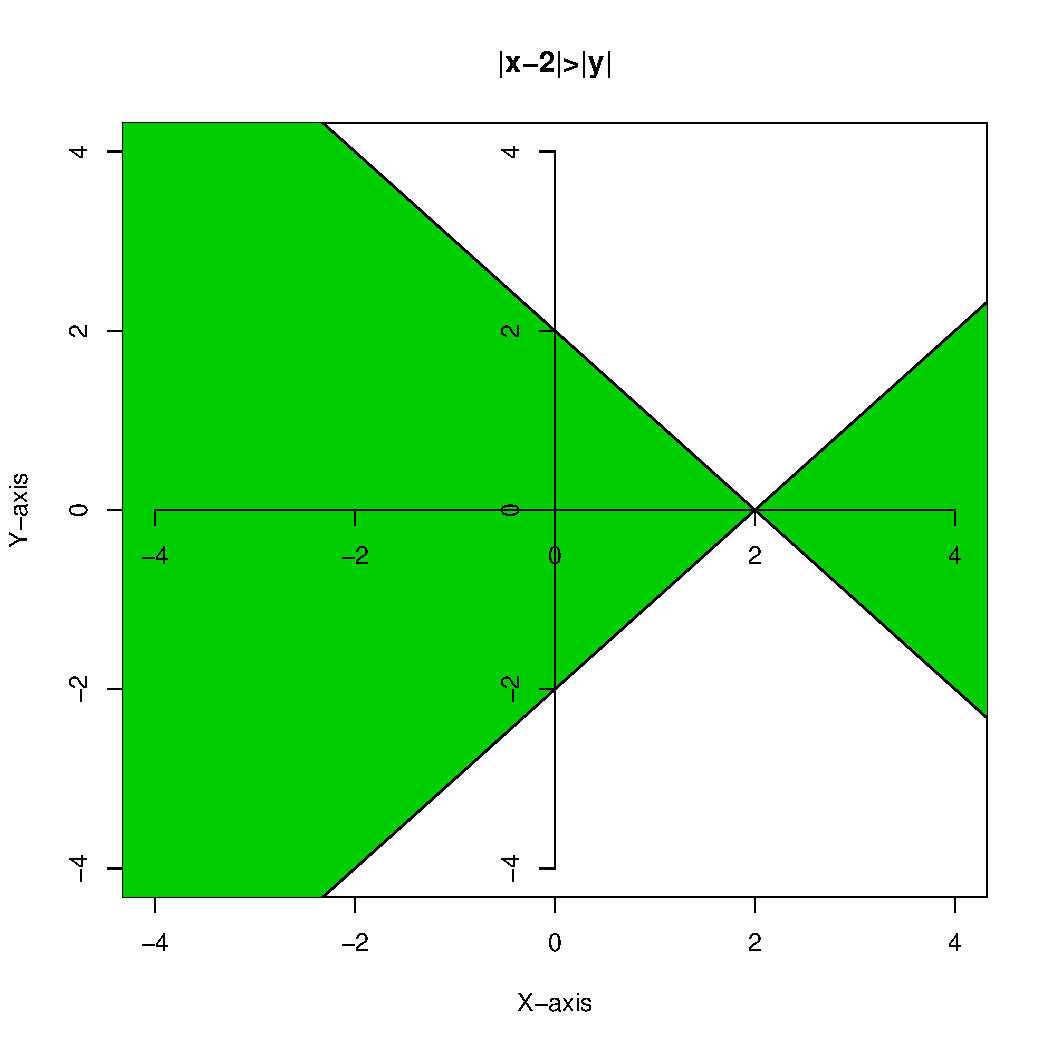
\includegraphics[scale=0.4]{dom_1_1.pdf}
         \caption{$\lvert x-2 \rvert > \lvert y \rvert$}
         \label{f1-1}
        \end{minipage} &
        \begin{minipage}[c]{200pt}
         \centering
         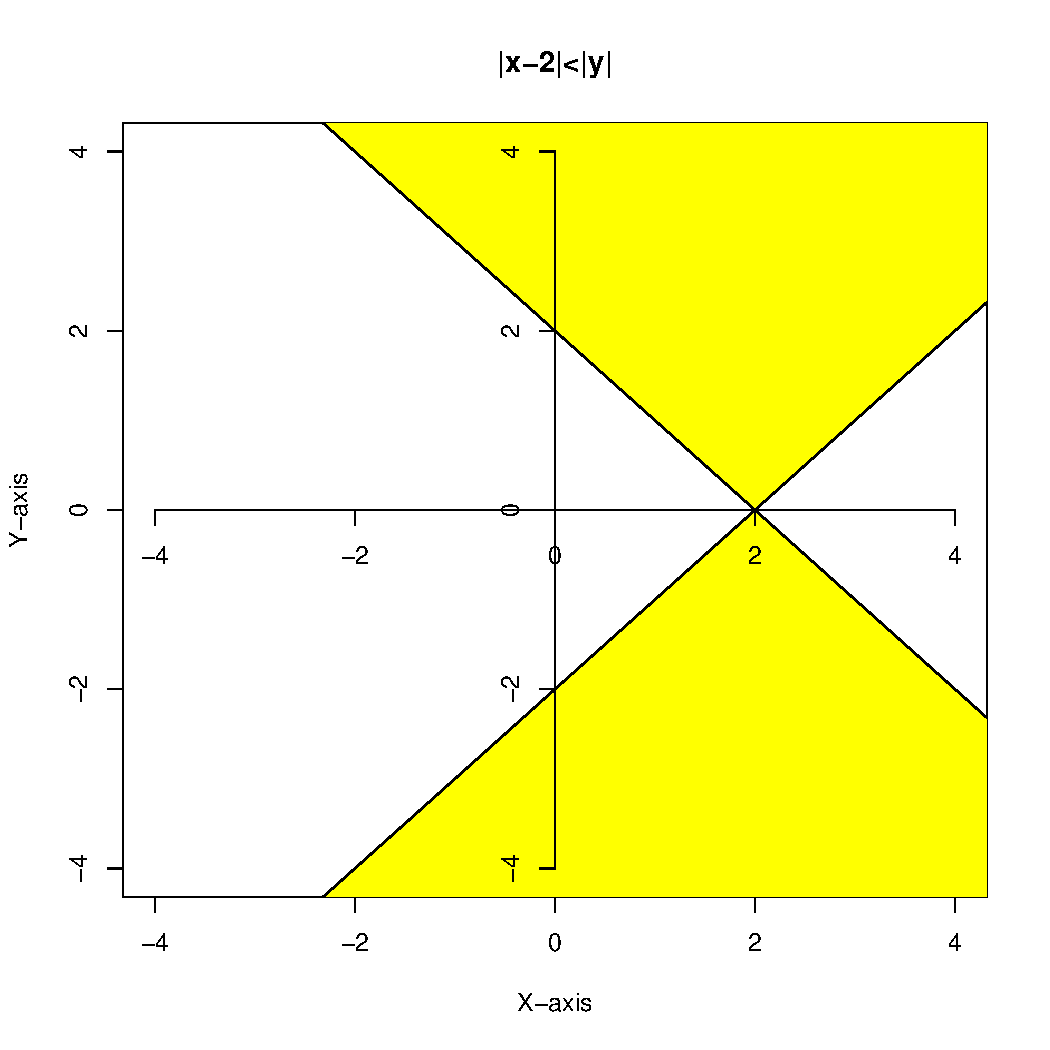
\includegraphics[scale=0.4]{dom_1_2.pdf}
         \caption{$\lvert x-2 \rvert \leq \lvert y \rvert$}
         \label{f1-2}
        \end{minipage} \\ \hline
        \begin{minipage}[c]{200pt}
         \centering
         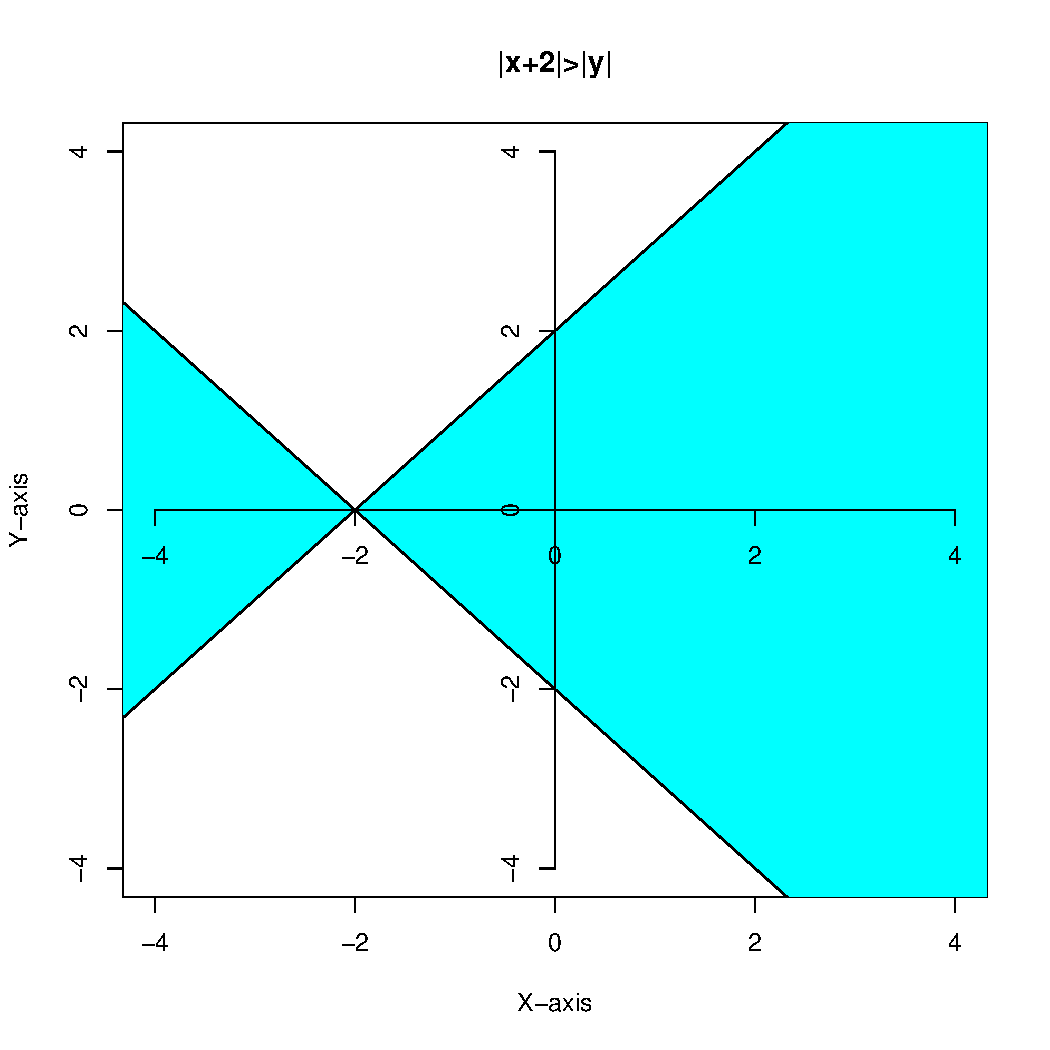
\includegraphics[scale=0.4]{dom_2_1.pdf}
         \caption{$\lvert x+2 \rvert > \lvert y \rvert$}
         \label{f2-1}
        \end{minipage} &
        \begin{minipage}[c]{200pt}
         \centering
         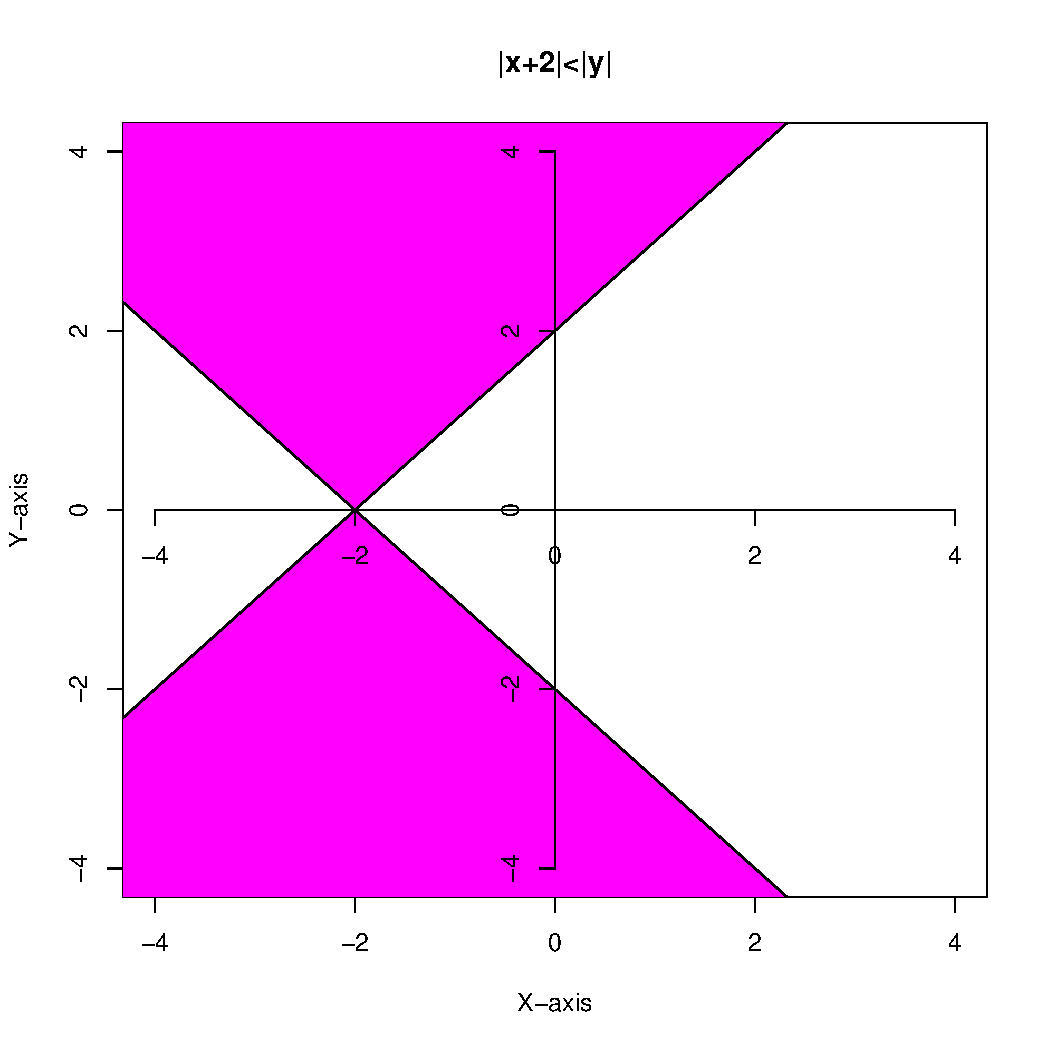
\includegraphics[scale=0.4]{dom_2_2.pdf}
         \caption{$\lvert x+2 \rvert \leq \lvert y \rvert$}
         \label{f2-2}
        \end{minipage}
       \end{tabular}
      \end{figure}


\end{enumerate}

\end{document}
